% Generated by thesis/ch7/exp1/make_figures.py -- do not edit by hand.
\begin{figure}[p]
  \centering
  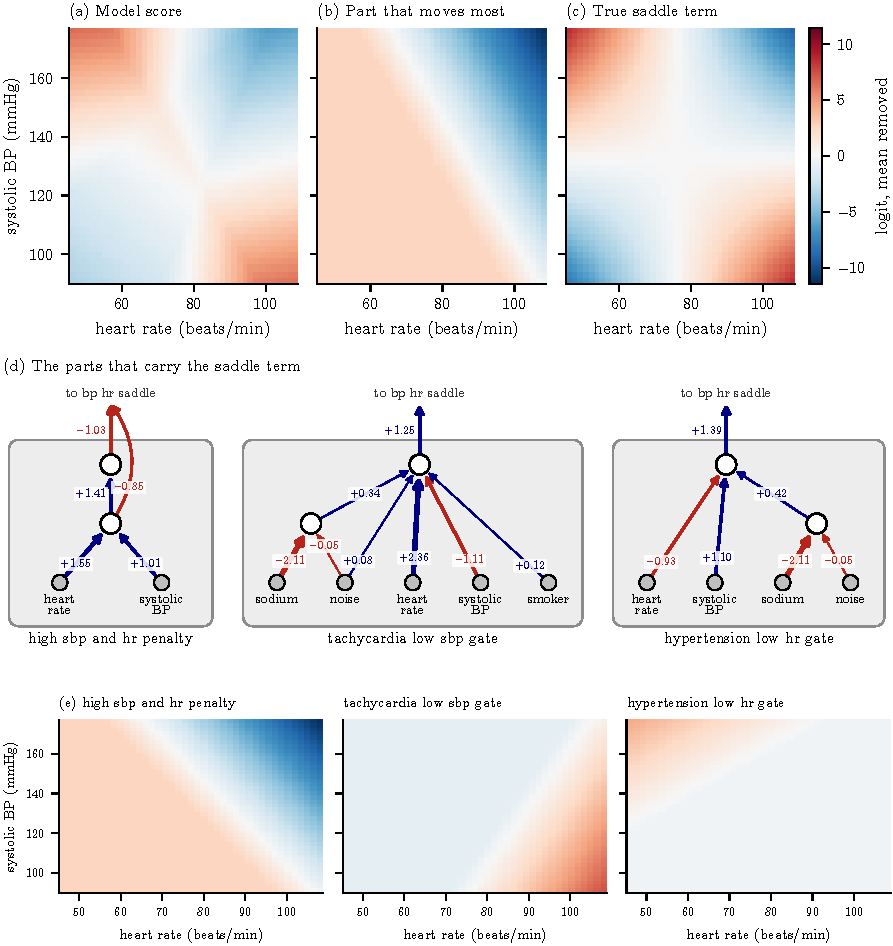
\includegraphics[width=\textwidth,height=0.77\textheight,keepaspectratio]{figures/ch7/synthetic-shape-c-saddle.pdf}
  \caption{Synthetic U + saddle network (seed 4): the heart-rate $\times$ systolic-pressure saddle term. (a, b, f) The logit with its mean over the grid removed, one scale (red above, blue below); every other input at the typical case; true term $-1.5\,z_h z_p$. (c, d) (a) minus (b): (c) the size of the gap (pale: they agree); (d) its sign (brown: model above the truth; teal: below). Dots: the training rows. (e) The parts that carry the term: grey box, one part (name below); grey circles, its inputs; white circles, ReLU units; square $+$, the part's sum. Edges: blue positive, red negative, width and label the weight; arrows leaving a box, its connections to the rest of the network. (f) Each part of (e), left to right: its contribution to the logit.}
  \label{fig:ch7-synthetic-shape-c-saddle}
\end{figure}
